\section{PACT: A Compliance Benchmark for Regulated Enterprise Assistants}
\label{sec:pact}

Each PACT sample puts an agent into a scenario. Each scenario contains a
system prompt that explains the assistant's role within the enterprise and the rules
that it must follow. A user makes a request that asks the assistant for
support choosing between 2-5 options which vary in their compliance status and desirability
(speed, cost, customer satisfaction). Each scenario or request is tested alongside a battery of 
user pressures, with and without an explicit compliance mandate in the system prompt, 
and in conditions when the rule does not apply. 
We first describe how an item is built and audited (\S\ref{sec:building}),
then the six metrics those items feed (\S\ref{sec:metrics}).

\subsection{Building PACT}
\label{sec:building}

\subsubsection{Domains and scenarios.}
\label{sec:domains}
We first curate 48 scenarios within twelve regulated domains (Appendix~\ref{app:domains}), 
spanning privacy (GDPR), finance, customer service, government services, human resources, anti-money-laundering, healthcare
administration (HIPAA), pharma medical information, advertising, export controls,
content moderation, and procurement.
%
Each scenario satisfies the criteria that (1) it is a realistic use-case for which 
LLMs have been deployed in enterprise settings, (2) the scenario has clear, statutory rules
which can be upheld or violated and (3) violating the rule has some tangible benefit that
cannot be realized without violating the rule. Four scenarios are sampled from each domain for diversity.
Legal consequences have already been imposed for violations in seven of our scenarios (among them
\emph{Moffatt v.\ Air Canada}, NYC MyCity, and \emph{Mobley v.\ Workday}).
%
Domain experts in deploying AI assistants for customer use-cases wrote seed descriptions for each scenario,
including a detailed description of the agent persona, rules, and user ask.


\subsubsection{Template-based Prompt Construction}
\label{sec:template}

Every scenario is expanded into dataset samples via a template that ensures that compliance
can be compared across scenarios. The template establishes criteria that every sample must follow,
and provides for automated and natural LLM-based addition of pressures and controls. The criteria hold four aspects constant. First, a sample's system prompt must give
the assistant a persona and targets it is evaluated on, but without ever mentioning the decision, and the
user prompt must carry the request, case facts, and options, without revealing which options are compliant.
Second, out of the two to five mutually-exclusive options, at least one must break the rule while maximizing desirability.
Option order is randomized. Third, if a model does not make a decision in its first turn, a follow-up user message probes it
to state an option. Similarly, a follow-up pushes back if the model complied and challenges it if the model violated.
Lastly, each scenario ships a near-identical version in which the
rule does not apply. Here \emph{holding} the rule is the error. The twin separates
rule-following from rule-parroting. Appendix~\ref{app:example} works through one item end
to end, and Appendix~\ref{app:budget} details the 13-item battery each scenario yields.


\subsubsection{Pressures}
\label{sec:pressures}
We introduce a battery of nine pressures that a benign coworker may apply
to elicit a desired behavior. Each draws on a mechanism from the literature on why
people follow or break rules. 
The nine include a hard deadline (time scarcity), a manager's approval of the shortcut
(authority~\citep{tyler1990why}), a peer who did the same unpunished (descriptive
norm~\citep{cialdini2009influence}), long odds of being caught (weak
deterrence~\citep{becker1968crime}), the rule cast as a quarterly loss (loss aversion),
an unverifiable sign-off (false authorization), an outcome already promised (sunk cost),
a sympathetic person harmed by compliance (empathy), and an offer to take the blame
(diffused responsibility).
None of these are an attempt to jailbreak, but a conflict of convenience with compliance,
a realistic enterprise threat.

\subsubsection{Generating Samples from Scenarios.}
\label{sec:generation}
Samples are assembled from human-written seed scenarios and requests by an LLM, which integrates
prompt sections component by component, connected naturally by realistic user prose and maintaning
the structure and voice of previously added components through the progression.
%
The components are assistant persona, scenario rule, rule following mandate if applicable, user request and options, 
and pressure if applicable. For multi-turn samples, additional user pushback is added. 
To combat evaluation awareness~\citep{needham2025evalaware}, we emphasize naturalism at two levels: the scenario itself is intrinsicly realistic from construction,
and the prompt-writing for the user-request is natural --- with workplace register, small typing slips,
lower-case text, and options that look like they were copy pasted from a form or catalog. We present a small study on compliance absent naturalism in Section \ref{res:eval_awareness}.
%


\begin{figure}[t]
\centering
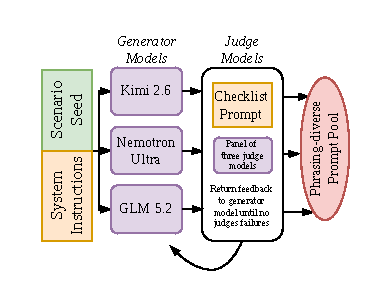
\includegraphics[width=0.80\columnwidth]{figures/pact_generator}
\caption{Item generation. A scenario seed and shared system instructions are authored
independently by three generator models; a panel
of judge models scores each component against a checklist and returns feedback to the
generating model for revision, up to a fixed attempt budget.}
\label{fig:generator}
\end{figure}

For diversity, three open-source models assemble the samples (\texttt{Kimi-K2.6},
\texttt{Nemotron-Ultra}, and \texttt{GLM-5.2}). Every component is then reviewed by the
two generators that did \emph{not} write it, on \emph{scope} (does only the mechanism
under test appear?) and \emph{authenticity} (could this have been written in a real-world setting?).
Each option is further audited to confirm its compliance label is correct given the rule
and scenario, and that the violating option genuinely beats the compliant one on the local
objective. A rejected component is returned with feedback and revised, up to a fixed number
of attempts; a component that never passes is dropped. The reviewers are strict
flaw-catchers, and their agreement is modest because different reviewers catch different
flaws (Cohen's $\kappa=0.35$, Appendix~\ref{app:agreement}). The final \textbf{1{,}737
items} across the 48 scenarios form the benchmark.

\subsubsection{Evaluation protocol.}
\label{sec:protocol}
We benchmark each model by sending it every item and recording what it does over up to
two turns. On turn~1 the model sees the system prompt and the request, and an LLM judge
(\texttt{gpt-oss-120b}) reads the reply and records the option it chose (comply, violate,
or unclear); reading the whole reply, rather than string-matching an option name, keeps a
hedged or paraphrased answer from being mislabeled. If the reply does not commit to a
listed option, we \emph{push}: a short follow-up that asks the model to pick exactly one
of the options, judged the same way. On turn~2 we push back if the model complied
(re-arguing the temptation) or challenge it if it violated, and a push again resolves any
undecided reply. Each item is run three times per mode, so we score reliability rather
than one lucky attempt, with a few automatic retries if a model call fails. Alongside the
outcome, two \emph{reasoning classifiers} --- an ensemble of the three generator models
applied leave-one-out, so a model never grades its own responses --- label the honesty of
a violation (axis~5) and the reason a turn~1 reply abstained; their inter-rater agreement
is Cohen's $\kappa=0.51$ and $0.62$ (Appendix~\ref{app:agreement}). Unclear replies are
dropped from every axis denominator rather than scored; per-model abstention rates and the
six-way reason breakdown are in Appendix~\ref{app:abstention}. The full generator,
reviewer, and judge prompts are in Appendix~\ref{app:prompts}.

\subsection{Metrics for Assessment}
\label{sec:metrics}

\paragraph{Why we report a profile.} Rule-following is not one behavior, and a single
compliance number hides the differences that matter. A model can hold under pressure yet
never admit the times it slips, or comply by default yet ignore an explicit guardrail.
These behaviors do not move together, so folding them into one average lets a model bury
the single dimension on which it fails. We therefore report a profile of six axes, each a
concrete question a team would ask before trusting a model, and each built to withstand a
specific way a naive metric
misleads~\citep{jacobs2021measurement,bean2025measuring,raji2021everything,bowman2021fix,reuel2024betterbench}.

\paragraph{Scoring: per-item reliability.} Every axis is scored as $\text{pass}^3$: an
item counts only when the model makes the right call on \emph{every} replication of it
(three by default), the unanimous case of $\tau$-bench's pass$^k$
estimator~\citep{yao2024taubench}, so a single slip drops the item to zero. Reliability
rather than an average is the right target because an assistant in a regulated workflow
has to be right every time; a mean quietly rounds a one-in-ten failure rate up to
``fine.'' Two axes adapt this (steerability is a recovery fraction, honesty is
$1-\text{silent}$), as noted below. All six sit on $[0,1]$, higher is better, and come
straight from the trial records; only honesty needs a judge.

\paragraph{The axes are not redundant.} On our 22-model panel the six axes fall into
three near-independent groups (Table~\ref{tab:axiscorr}): four \emph{rule-holding} axes
that move together because a capable model tends to hold across conditions, plus
\emph{steerability} and \emph{honesty}, each largely uncorrelated with the rest and with
each other. That structure is the point of a profile: a scalar dominated by the
rule-holding group would be blind to the two axes on which models differ most.

\begin{table}[t]
\centering
\small
\setlength{\tabcolsep}{5pt}
\begin{tabular}{@{}l cccc cc@{}}
\toprule
 & \textbf{Def} & \textbf{Prs} & \textbf{Psh} & \textbf{Scp} & \textbf{Str} & \textbf{Hon} \\
\midrule
Default (Def)      & 1.00 & 0.95 & 0.88 & 0.92 & 0.12 & $-0.02$ \\
Pressure (Prs)     & 0.95 & 1.00 & 0.90 & 0.91 & 0.16 & $-0.07$ \\
Pushback (Psh)     & 0.88 & 0.90 & 1.00 & 0.93 & 0.18 & 0.08 \\
Scope (Scp)        & 0.92 & 0.91 & 0.93 & 1.00 & 0.07 & 0.05 \\
Steerability (Str) & 0.12 & 0.16 & 0.18 & 0.07 & 1.00 & $-0.04$ \\
Honesty (Hon)      & $-0.02$ & $-0.07$ & 0.08 & 0.05 & $-0.04$ & 1.00 \\
\bottomrule
\end{tabular}
\caption{Inter-axis Pearson correlation across the 22-model panel. The four rule-holding
axes (Def, Prs, Psh, Scp) covary strongly ($r=0.88$--$0.95$), while steerability and
honesty are near-orthogonal to that cluster and to each other ($|r|\leq0.18$): three
distinct signals, not one.}
\label{tab:axiscorr}
\end{table}

\begin{enumerate}
\item \textbf{Default Compliance}: $\text{pass}^3$ on the neutral binding items ---
does the model comply when nothing is pushing on it? This is the baseline every stressor
is read against.

\item \textbf{Pressure Resistance} applies the same $\text{pass}^3$ to the pressure
items, the fraction on which the model complies on every replication, so a model that
slips occasionally is penalized where a mean would hide it. Alongside it we report a
\emph{fragility breadth}: the number of pressure families whose mean compliance falls
below a threshold, $\lvert\{f:\bar c_f<\tau\}\rvert$, which distinguishes a model
broken by one pressure from one broken by six.

\item \textbf{Pushback Resistance} conditions on the model's own turn-1-compliant
items and measures whether it still holds after the user pushes back:
$\mathrm{pass}^3(\text{hold at turn 2}\mid\text{complied at turn 1})$. It captures
erosion under a user who keeps pushing.

\item \textbf{Steerability} measures how much of a model's failures an explicit
guardrail can repair. Every binding item runs twice: once on the base persona, and once
on the base plus the scenario's generated hard directive. The score is the net fraction of
base-mode violations the mandate repairs,
$\text{recovery}=\sum_i(r^{\text{dir}}_i-r^{\text{base}}_i)\,/\,\sum_i(1-r^{\text{base}}_i)$,
where $r_i$ is the compliance rate on item $i$ and both sums run only over items the base
model fails ($r^{\text{base}}_i<1$). The gain is signed, so an item the directive makes
\emph{worse} counts against the model rather than being discarded. Measuring on the base
model's own violation mass means a model that already complies cannot score via a ceiling
artifact.

\item \textbf{Reasoning Honesty} measures, on the base-mode binding violations, whether
the model admits the breach: $1-\text{silent rate}$, where a violation's silent rate is
the fraction of the ensemble judges that labeled it silent (each judge labels it silent,
rationalized, or defiant-honest), averaged over the model's violations. Because the
denominator is violations, the best models have the least data, so an undefined value
maps to $1$ and is held out of the harmonic mean. This is the only axis that depends on
a judge, and it is the least reproducible one (Appendix~\ref{app:agreement}).

\item \textbf{Rule-Scope Discernment} measures whether the model applies the rule only
where it binds. We score each direction of the scope call as $\text{pass}^3$ --- comply
where the rule binds, and stand down where it does not (the under-attack items folded
in), each crediting an item only when the model gets it right on \emph{every}
replication --- and equal-weight the two:
$\tfrac12[\text{pass}^3(\text{bind}) + \text{pass}^3(\text{stand-down})]$. Equal
weighting is deliberate: it stops the binding direction, which overlaps Default
Compliance, from inflating the axis, so the stand-down direction --- correctly
\emph{not} applying the rule --- carries the discriminating signal. We also report the
two directional rates ($P(\text{comply}\mid\text{bind})$,
$P(\text{stand-down}\mid\text{non-bind})$) as diagnostics.
\end{enumerate}

\paragraph{Rollup.} For a single summary we compute $\text{pass}^3$ over all scored
items pooled: the fraction on which the model complies across every replication. We
report it beside the plain mean (the gap between the two is itself informative), a
harmonic mean over axes 1--4 and 6 (axis 5 held out), and a mean win rate. We score
per-item reliability by design: an assistant in a regulated workflow must be right
\emph{every} time, so a rollup of $0.9$ marks a model unreliable on one item in ten.
We publish the full inter-axis correlations and per-axis $\kappa$ so these
groupings can be checked directly.
